\documentclass{ximera}
\usepackage{OERLinearAlgebra}


\usepackage{mathtools}
\usepackage{tikz-3dplot}
\newcommand\norm[1]{\left\lVert#1\right\rVert}

\author{Anna Davis \and Rosemarie Emanuele} \title{Length of a Vector} \license{CC-BY 4.0}

\begin{document}

\begin{abstract}
 We find vector magnitude.
\end{abstract}
\maketitle
\vskip 5pt


Vector quantities, such as velocity and force, have magnitude and direction.  The magnitude of a vector quantity is the length of the vector.  For example, if a force of 10 Newtons is applied to an object, we would represent the force by a 10-unit-long vector.

 \begin{image}[2in]
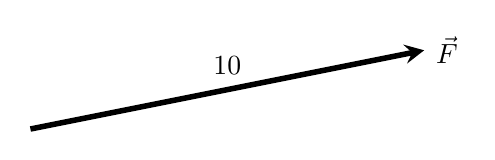
\begin{tikzpicture}[scale=1]
\draw[line width=2pt,-stealth](0,0)--(5,1)node[right]{$\vec{F}$} ;
\node[] at (2.5, 0.8)   {$10$};
\end{tikzpicture}
\end{image}

The magnitude of a vector is denoted by double absolute value brackets.  In the case of force $\vec{F}$, we write $$\norm{\vec{F}}=10$$

To find the length of a vector, we need to find the distance between the tail of the vector and its head.  Recall that in $\RR^2$, the distance between $A(a_1, a_2)$ and $B(b_1, b_2)$ is given by 
\begin{equation*}
d_{AB}=\sqrt{(a_1-b_1)^2+(a_2-b_2)^2}
\end{equation*}
A vector $\vec{v}=[v_1, v_2]$ has the length of  a vector in standard position with its head at $(v_1, v_2)$ and tail at $(0, 0)$. We find the length of $\vec{v}$ using the distance formula

\begin{equation}\label{eq:normr2}
\norm{\vec{v}}=\sqrt{(v_1-0)^2+(v_2-0)^2}=\sqrt{v_1^2+v_2^2}
\end{equation}

\begin{example} Find the magnitude of $\vec{u}=[-3,4]$.  
\begin{image}[1.8in]
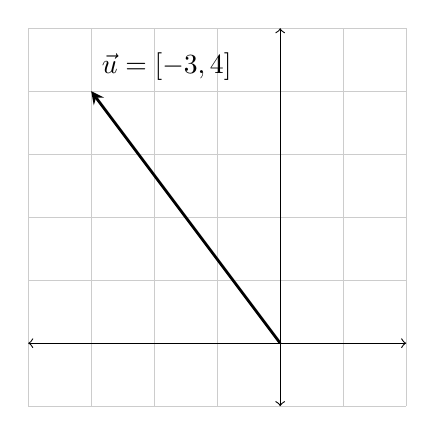
\begin{tikzpicture}[scale=0.8]
\draw[thin,gray!40] (-4,-1) grid (2,5);
  \draw[<->] (-4,0)--(2,0);
  \draw[<->] (0,-1)--(0,5);
  \draw[line width=1pt,-stealth](0,0)--(-3,4) node[above right]{$\vec{u}=[-3,4]$};
 \end{tikzpicture}
\end{image}
\begin{explanation}

 $$
\norm{\vec{u}}=\sqrt{(-3)^2+(4)^2}=5
$$
\end{explanation}
\end{example}


The distance formula for points in $\RR^3$ is analogous to the distance formula in $\RR^2$.  Given two points $A(a_1, a_2, a_3)$ and $B(b_1, b_2, b_3)$, the distance between them is given by 

\begin{equation*}
d_{AB}=\sqrt{(a_1-b_1)^2+(a_2-b_2)^2+(a_3-b_3)^2}
\end{equation*}

To find the length of vector $\vec{v}=[v_1, v_2, v_3]$, we find the distance between $(v_1, v_2, v_3)$ and $(0, 0, 0)$.
\begin{equation}\label{eq:normr3}
\norm{\vec{v}}=\sqrt{(v_1-0)^2+(v_2-0)^2+(v_3-0)^2}=\sqrt{v_1^2+v_2^2+v_3^2}
\end{equation}

\begin{example}
The magnitude of $\vec{v}=[6,-2,3]$ is given by
$$
\norm{\vec{v}}=\sqrt{(6)^2+(-2)^2+(3)^2}=7
$$
\end{example}


Distance formulas for $\RR^2$ and $\RR^3$ motivate the following definition of distance between two points in $\RR^n$.

  \begin{definition}[Distance Between Two Points in $\RR^n$] \label{def:distrn} Let $A(a_1, a_2,\ldots, a_n)$ and $B(b_1, b_2,\ldots, b_n)$ be points in $\RR^n$.  The distance between $A$ and $B$ is defined by 
\begin{equation*}
d_{AB}=\sqrt{(a_1-b_1)^2+(a_2-b_2)^2+\ldots +(a_n-b_n)^2}
\end{equation*}
\end{definition}

The following definition follows directly from the distance formula for $\RR^n$ in the same way that expressions (\ref{eq:normr2}) and (\ref{eq:normr3}) followed from distance formulas in $\RR^2$ and $\RR^3$.  
\begin{definition}[Magnitude of a Vector in $\RR^n$]\label{def:normrn}
Let $\vec{v}=[v_1, v_2, \ldots ,v_n]$ be a vector in ${\bf R}^n$, then
\begin{equation} \label{eq:normrn}
\norm{\vec{v}}=\sqrt{v_1^2+v_2^2+\ldots +v_n^2}
\end{equation}
\end{definition}

\begin{example}
The magnitude of $\vec{w}=[5, -1, -2, 4]$ is given by
 $$\norm{\vec{w}}=\sqrt{5^2+(-1)^2+(-2)^2+4^2}=\sqrt{46}$$ 
\end{example}

\section*{Practice Problems}
\begin{problem}
Find the length of the following vectors.  Enter your answers in exact, simplified form.
\begin{enumerate}
\item
 $$\vec{u}=[1,3]$$ 
 Answer:
 $$\norm{\vec{u}}=\sqrt{\answer{10}}$$
 \item
 $$\vec{v}=[-4,-6]$$
 Answer:
 $$\norm{\vec{v}}=\answer{2}\sqrt{\answer{13}}$$
 \item
 $$\vec{w}=[2,-4,6]$$
 Answer:
 $$\norm{\vec{w}}=\answer{2}\sqrt{\answer{14}}$$
 \item
 $$\vec{q}=[-10, 4, -7, 5, 3]$$
 Answer:
 $$\norm{\vec{q}}=\sqrt{\answer{199}}$$
 \end{enumerate}
 \end{problem}
 
\begin{problem}
Find the component form of vector $\vec{v}$ in $\RR^2$ if we know that $\norm{\vec{v}}=15$, the $x$ component of $\vec{v}$ is $-9$ and the vector is located in the third quadrant.

Answer:
$$\vec{v}=[-9,\answer{-12}]$$
\end{problem}

\begin{problem}
For a vector in $\RR^2$ with a length of 26 and the $y$ component of 10, what are the possibilities for the $x$ component?  List the possibilities in an increasing order.

Answer:
$$\answer{-24},\quad\text{and}\quad\answer{24} $$
\end{problem}

\begin{problem}
Let $\vec{v}=[1, y, 4]$.  Find all possible values of $y$ if $\norm{\vec{v}}=9$.  List the possibilities in an increasing order.

Answer:
$$\answer{-8},\quad\text{and}\quad\answer{8}$$
\end{problem}

\begin{problem}
For a vector in $\RR^4$, what are the possibilities for the fourth component if the length of the vector is 14, and the $x$, $y$ and $z$ components are 1, 5 and 13, respectively? List the possibilities in an increasing order.

Answer:
$$\answer{-1},\quad\text{and}\quad\answer{1}$$
\end{problem}
 
 



\end{document} 